\section{Results}
\label{sec:evaluation}

\subsection{Dataset Quality and Diversity}

\FloatBarrier

To assess the quality and structural diversity of datasets generated by QueryBloom, we compare a synthesized dataset against DBpedia QALD-9, a standard human-authored benchmark. We evaluate diversity across three dimensions: query feature complexity, semantic linguistic variety, and holistic schema coverage.


\textbf{Query Structural Complexity.} The distribution of SPARQL 1.1 operators within both datasets shows that QueryBloom demonstrates significantly higher structural complexity in several key dimensions compared to the QALD-9 baseline. Notably, QueryBloom queries incorporate \texttt{FILTER} constraints at roughly four times the rate of the baseline. Furthermore, they heavily utilize \texttt{OPTIONAL} blocks and property paths, which are entirely absent from the QALD-9 test set. Both datasets maintain a comparable usage of \texttt{UNION} operators. This confirms that QueryBloom maintains a higher level of structural complexity than the QALD-9 baseline which more closely reflects the complexity of real-world SPARQL queries.

\textbf{Semantic Linguistic Diversity.} To evaluate the natural language variety of the generated questions, we compute dense semantic embeddings for each question text using SBERT (BGE-large) and project these embeddings into a 2D space via t-SNE. We compute Average Pairwise Distance (APD) for global diversity and Mean Nearest-Neighbour Distance (MNND) for local density. QueryBloom achieves a higher APD and MNND, which indicates that QueryBloom successfully covers a wider semantic space of linguistic intents and vocabulary than the fixed human-authored QALD-9 test set.

\textbf{Holistic Schema Coverage.} We present a multi-dimensional summary of dataset diversity across five key metrics:
\begin{itemize}
    \item \textbf{Unique Entities \& Relations:} The average number of distinct entities and properties referenced per query, reflecting how broadly the dataset explores the underlying knowledge graph schema.
    \item \textbf{Variables \& Triples:} The median number of variables and triple patterns per query, measuring the structural size and depth of the generated SPARQL.
    \item \textbf{Unique Templates:} The ratio of distinct SPARQL skeletons (where specific entities, variables, and literals are anonymized) to the total number of queries, assessing syntactic novelty.
\end{itemize}

QueryBloom outperforms QALD-9 across almost all these dimensions. Most strikingly, it achieves a substantially higher unique template ratio, indicating that its SPARQL skeletons are even more diverse than those found in the human-authored benchmark. The next clearest difference is structural depth, with QueryBloom producing a median of roughly three times as many triple patterns per query as the baseline. Furthermore, it consistently incorporates a higher rate of unique entities per query, ensuring broader and more diverse coverage of the graph's instance data.

\begin{figure*}[p]
    \centering
    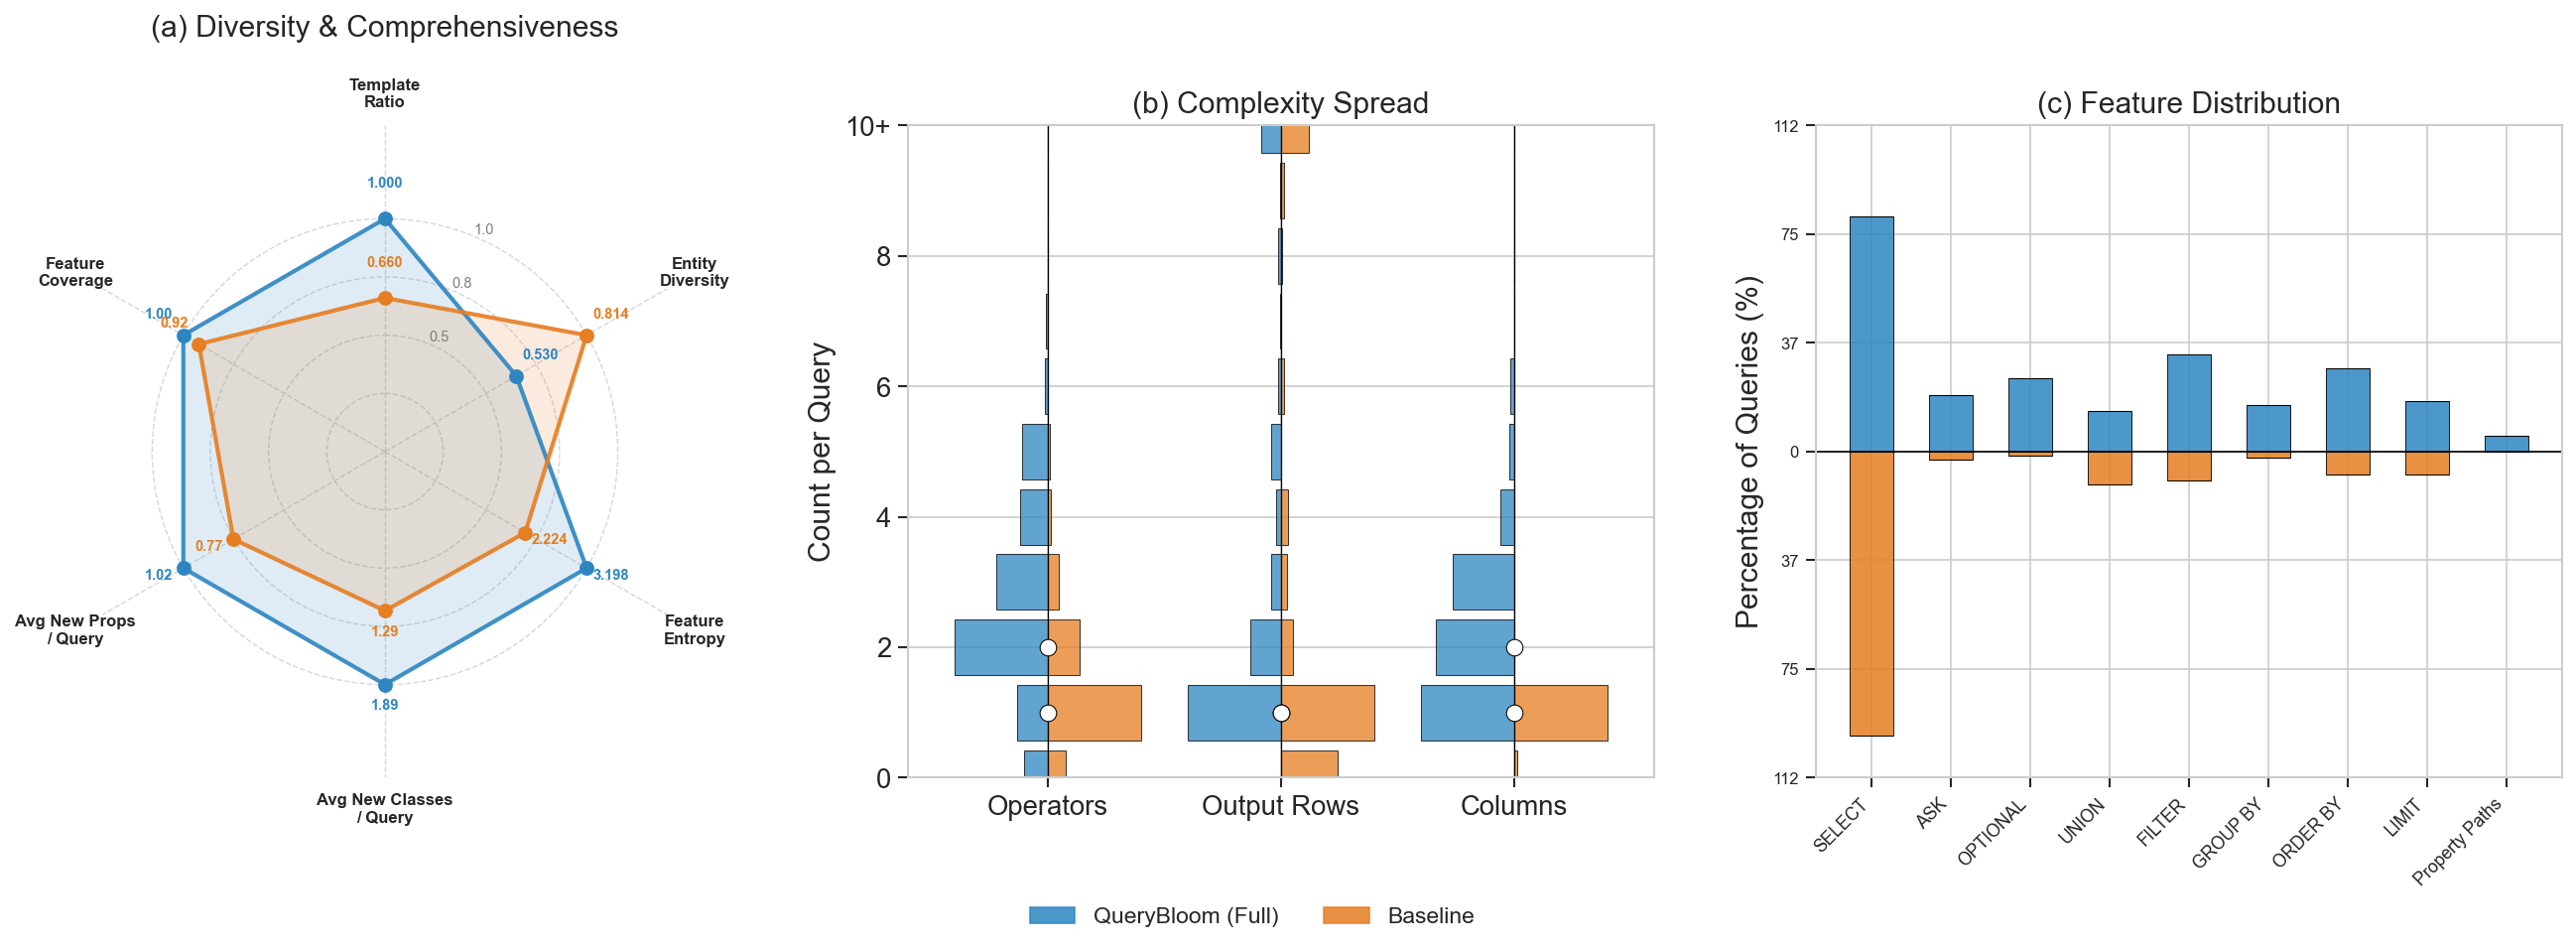
\includegraphics[width=\textwidth]{figures/eval/diversity-dbpedia.png}
    \par\medskip
    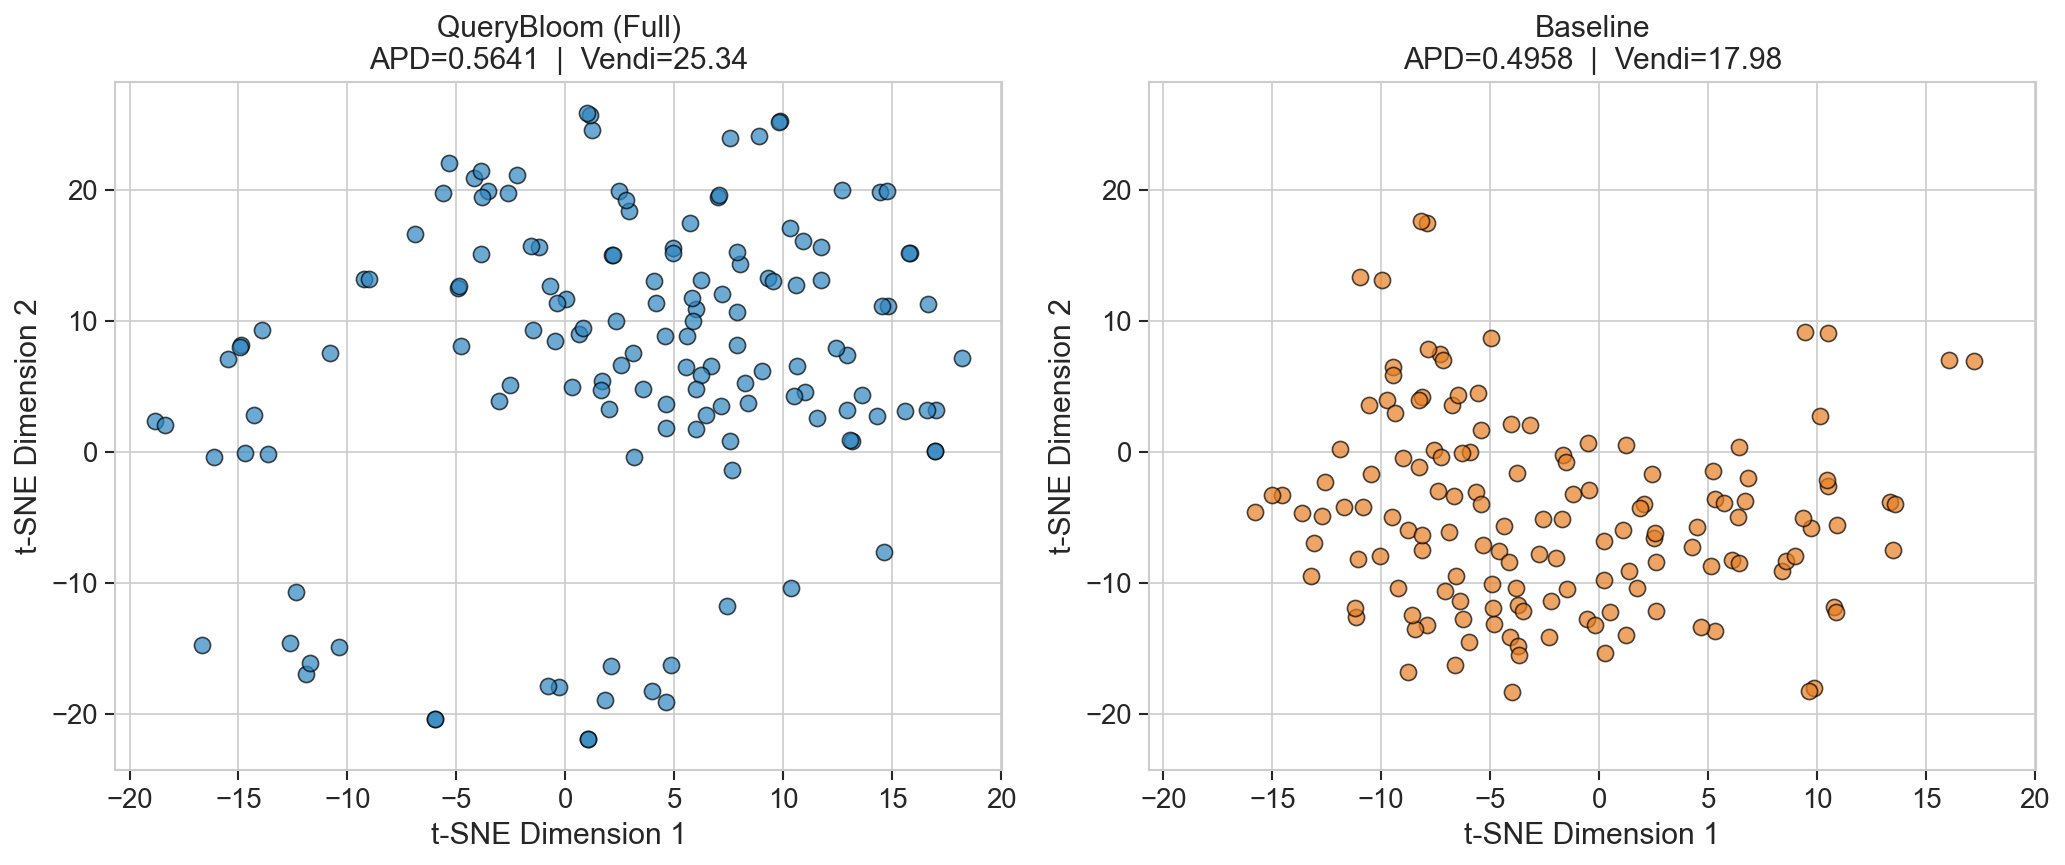
\includegraphics[width=\textwidth]{figures/eval/semantic-dbpedia.png}
    \caption*{DBpedia knowledge graph}
\end{figure*}
\clearpage

\begin{figure*}[p]
    \centering
    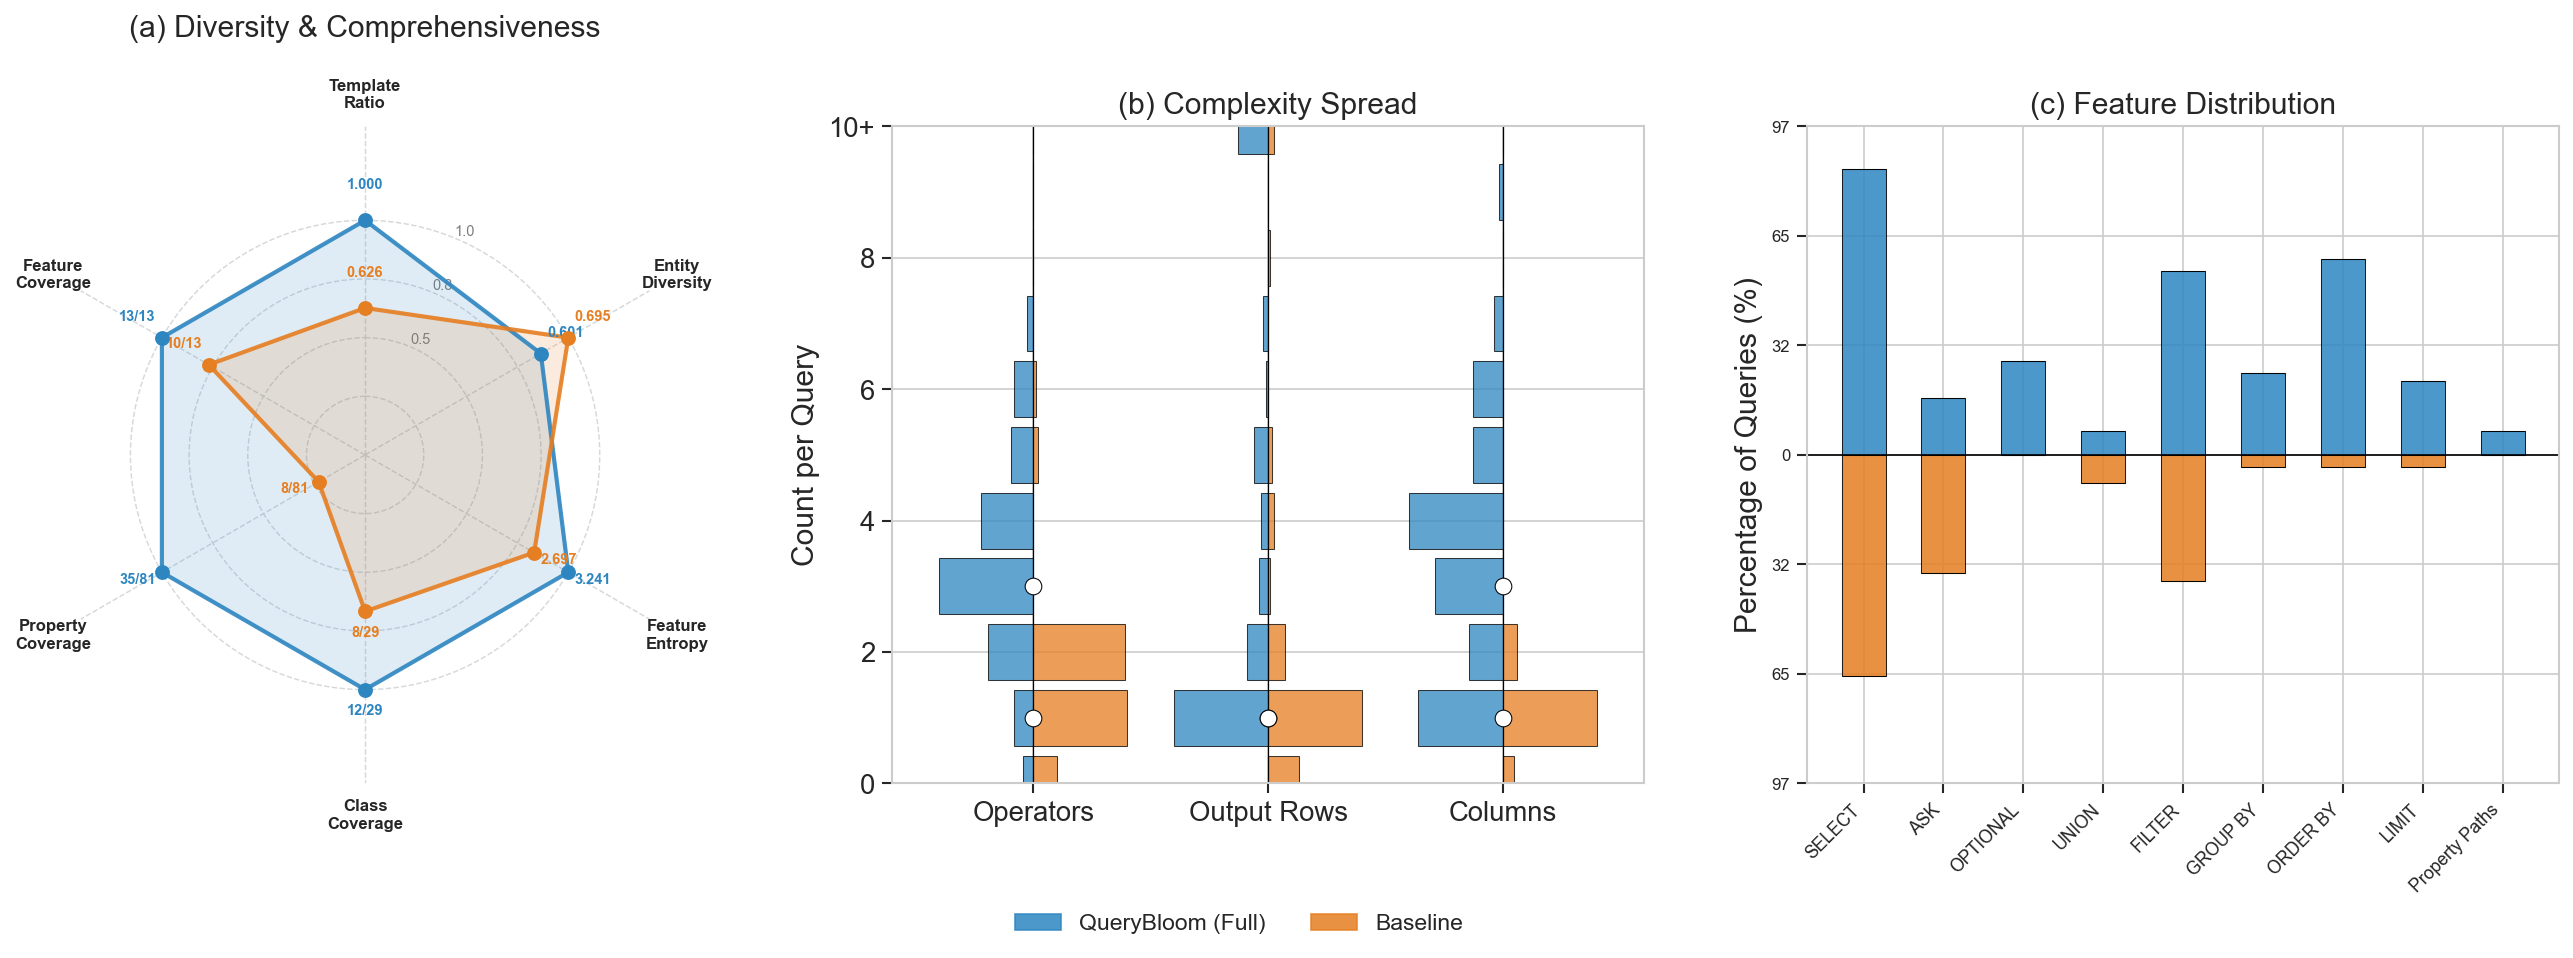
\includegraphics[width=\textwidth]{figures/eval/diversity-dblp.png}
    \par\medskip
    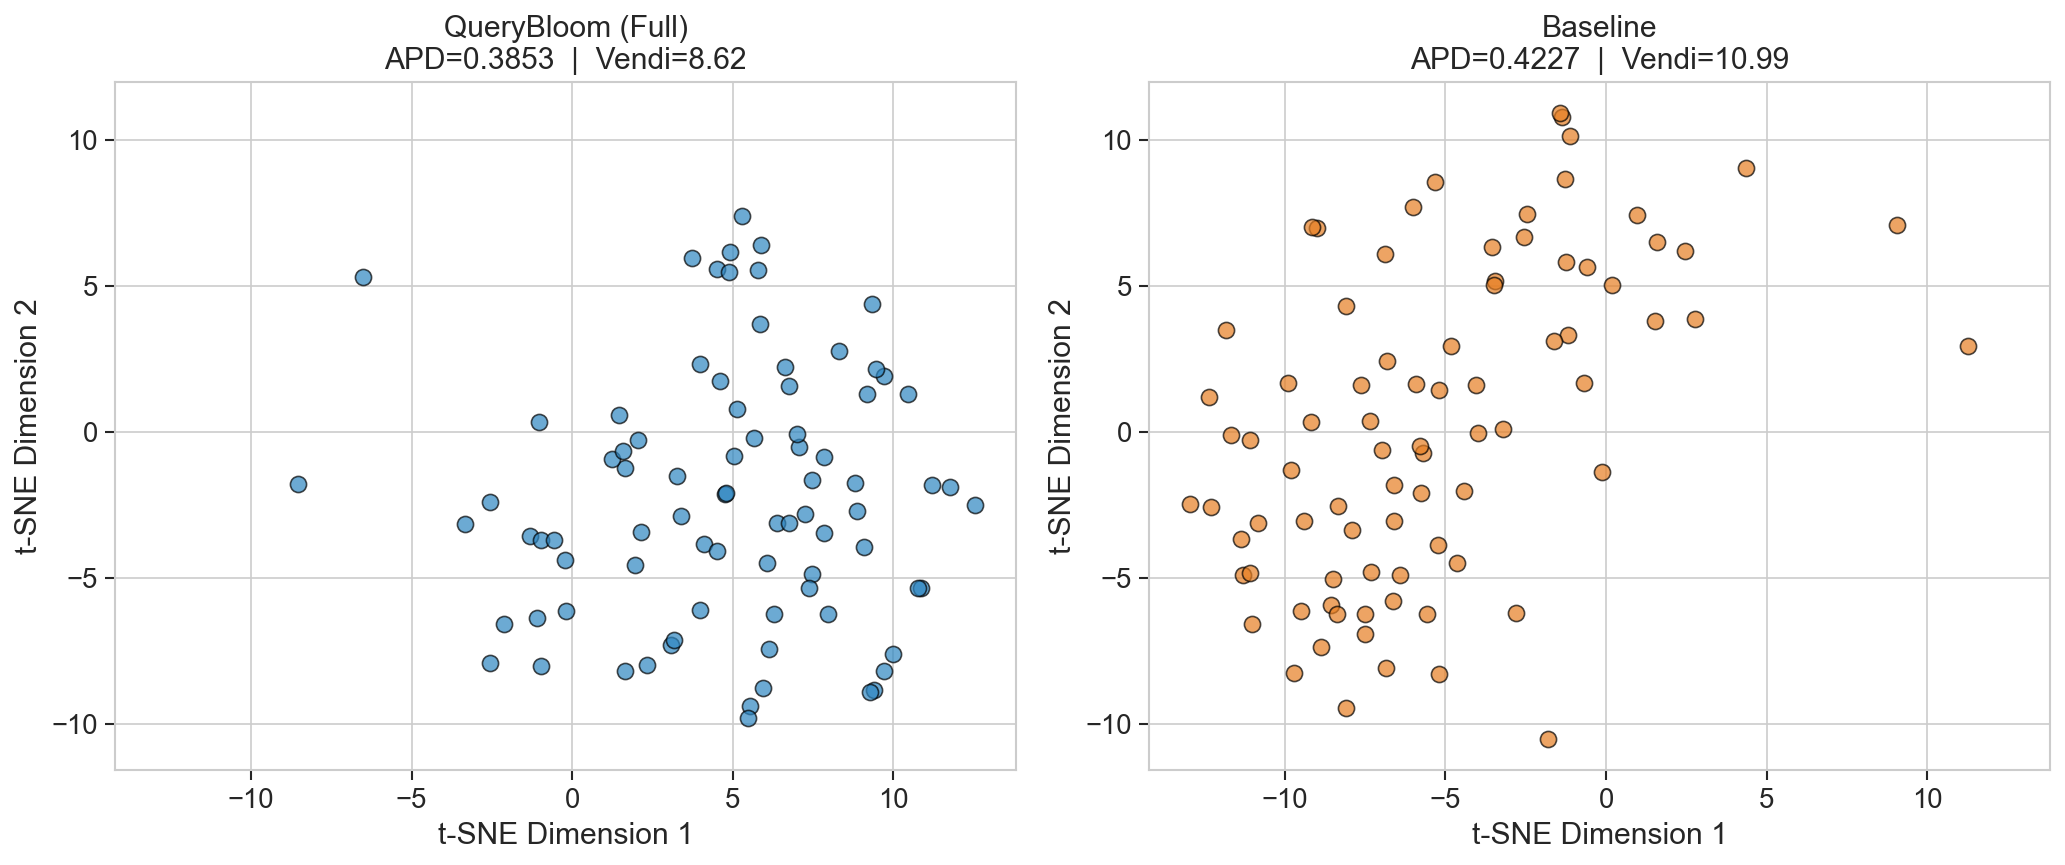
\includegraphics[width=\textwidth]{figures/eval/semantic-dblp.png}
    \caption*{DBLP knowledge graph}
\end{figure*}

\clearpage